%\refsection
\chapter{\texorpdfstring{Evoluzione dell'Infrastruttura Tecnologica: dalle Fondamenta Fisiche alle Architetture Moderne}{Capitolo 3 - Evoluzione dell'Infrastruttura Tecnologica: dalle Fondamenta Fisiche alle Architetture Moderne}}
\label{cap3_infrastructure_evolution}

\section{\texorpdfstring{Introduzione}{3.1 - Introduzione}}
\label{sec:cap3_intro}

L'analisi del panorama delle minacce presentata nel Capitolo 2 ha evidenziato come il 78\% degli attacchi informatici nel settore della Grande Distribuzione Organizzata (\gls{gdo}) sfrutti vulnerabilità architetturali piuttosto che debolezze nei singoli controlli di sicurezza\autocite{Anderson2024patel}. Questo dato fondamentale, derivato dall'analisi di oltre 1.200 incidenti documentati nel periodo 2020-2024, sottolinea l'importanza critica di un'architettura infrastrutturale robusta come prima linea di difesa\autocite{verizon2024}.

Il presente capitolo affronta l'evoluzione dell'infrastruttura tecnologica attraverso un percorso strutturato che parte dalle componenti fisiche fondamentali per arrivare alle moderne architetture distribuite. L'obiettivo principale consiste nel dimostrare come un'evoluzione pianificata dell'infrastruttura possa simultaneamente migliorare le prestazioni operative (con Accordi sul Livello di Servizio - \textbf{\gls{sla}} - superiori al 99,95\%) e ridurre significativamente i costi di gestione (con riduzioni del Costo Totale di Proprietà - \gls{tco} - superiori al 30\%)\autocite{IDC2024}.

\section{\texorpdfstring{Framework di Evoluzione Infrastrutturale}{3.2 - Framework di Evoluzione Infrastrutturale}}
\label{sec:framework_evoluzione}

\subsection{\texorpdfstring{Modello Teorico di Riferimento}{3.2.1 - Modello Teorico di Riferimento}}
\label{subsec:modello_teorico}

L'evoluzione delle infrastrutture tecnologiche nelle organizzazioni complesse come la \gls{gdo} segue un percorso che può essere descritto attraverso un modello di maturità a cinque livelli\autocite{Gartner2024hype}:

\begin{table}[htbp]
\centering
\caption{Livelli di Maturità Infrastrutturale nel settore \gls{gdo}}
\label{tab:maturity_levels}
\small
\sffamily
\begin{tabularx}{\textwidth}{c X c c}
\toprule
\textbf{Livello} & \textbf{Caratteristiche} & \textbf{Disponibilità} & \textbf{Costi Operativi} \\
\midrule
1. Tradizionale & Infrastruttura fisica isolata, gestione manuale & 95-97\% & Baseline (100\%) \\
2. Consolidato & Virtualizzazione parziale, primi sistemi di monitoraggio & 97-98,5\% & 85-90\% \\
3. Automatizzato & Orchestrazione dei servizi, gestione centralizzata & 98,5-99,5\% & 70-75\% \\
4. Ottimizzato & Architetture ibride, automazione avanzata & 99,5-99,9\% & 55-60\% \\
5. Adattivo & Infrastruttura intelligente, auto-riparazione & >99,95\% & 45-50\% \\
\bottomrule
\end{tabularx}
\end{table}

Il passaggio tra i diversi livelli di maturità non avviene in modo lineare ma richiede investimenti mirati e una strategia di trasformazione graduale. L'analisi empirica condotta su 47 organizzazioni europee del settore\autocite{eurostat2024} ha evidenziato che il tempo medio per progredire di un livello si attesta sui 14-18 mesi, con investimenti che variano tra il 15\% e il 25\% del budget IT annuale.

\section{\texorpdfstring{Infrastruttura Fisica: le Fondamenta della Resilienza}{3.3 - Infrastruttura Fisica: le Fondamenta della Resilienza}}
\label{sec:infrastruttura_fisica}

\subsection{\texorpdfstring{Sistemi di Alimentazione Elettrica}{3.3.1 - Sistemi di Alimentazione Elettrica}}
\label{subsec:alimentazione}

L'affidabilità dell'infrastruttura tecnologica dipende in primo luogo dalla continuità dell'alimentazione elettrica. I dati raccolti dal consorzio Uptime Institute\autocite{Uptime2024} mostrano che il 43\% delle interruzioni di servizio superiori alle 4 ore nel settore della distribuzione organizzata deriva da problemi nell'alimentazione elettrica, con costi medi di 127.000 euro per ogni ora di fermo durante i periodi di picco commerciale.

\subsubsection{\texorpdfstring{Architettura dei Sistemi di Continuità}{3.3.1.1 - Architettura dei Sistemi di Continuità}}

I sistemi di continuità elettrica (\textbf{\gls{ups}} - Uninterruptible Power Supply) rappresentano la prima linea di difesa contro le interruzioni. Nella \gls{gdo}, l'architettura standard prevede configurazioni ridondanti che garantiscono la continuità operativa anche in caso di guasti multipli\autocite{IEEE2024}.

La configurazione più diffusa, denominata N+1, prevede l'installazione di unità \gls{ups} aggiuntive rispetto al fabbisogno nominale. Per esempio, per un carico di 300 kW servito da unità da 100 kW ciascuna, si installano 4 unità invece delle 3 strettamente necessarie. Questa ridondanza garantisce una disponibilità teorica del 99,94\%.

Le organizzazioni più mature adottano invece una configurazione 2N, che prevede la duplicazione completa del sistema di alimentazione. Questo approccio, seppur più costoso (con un incremento dell'investimento iniziale del 40-50\%), garantisce la possibilità di effettuare manutenzioni programmate senza alcuna interruzione del servizio e tollera il guasto completo di un'intera catena di alimentazione.

\begin{figure}[htbp]
\centering
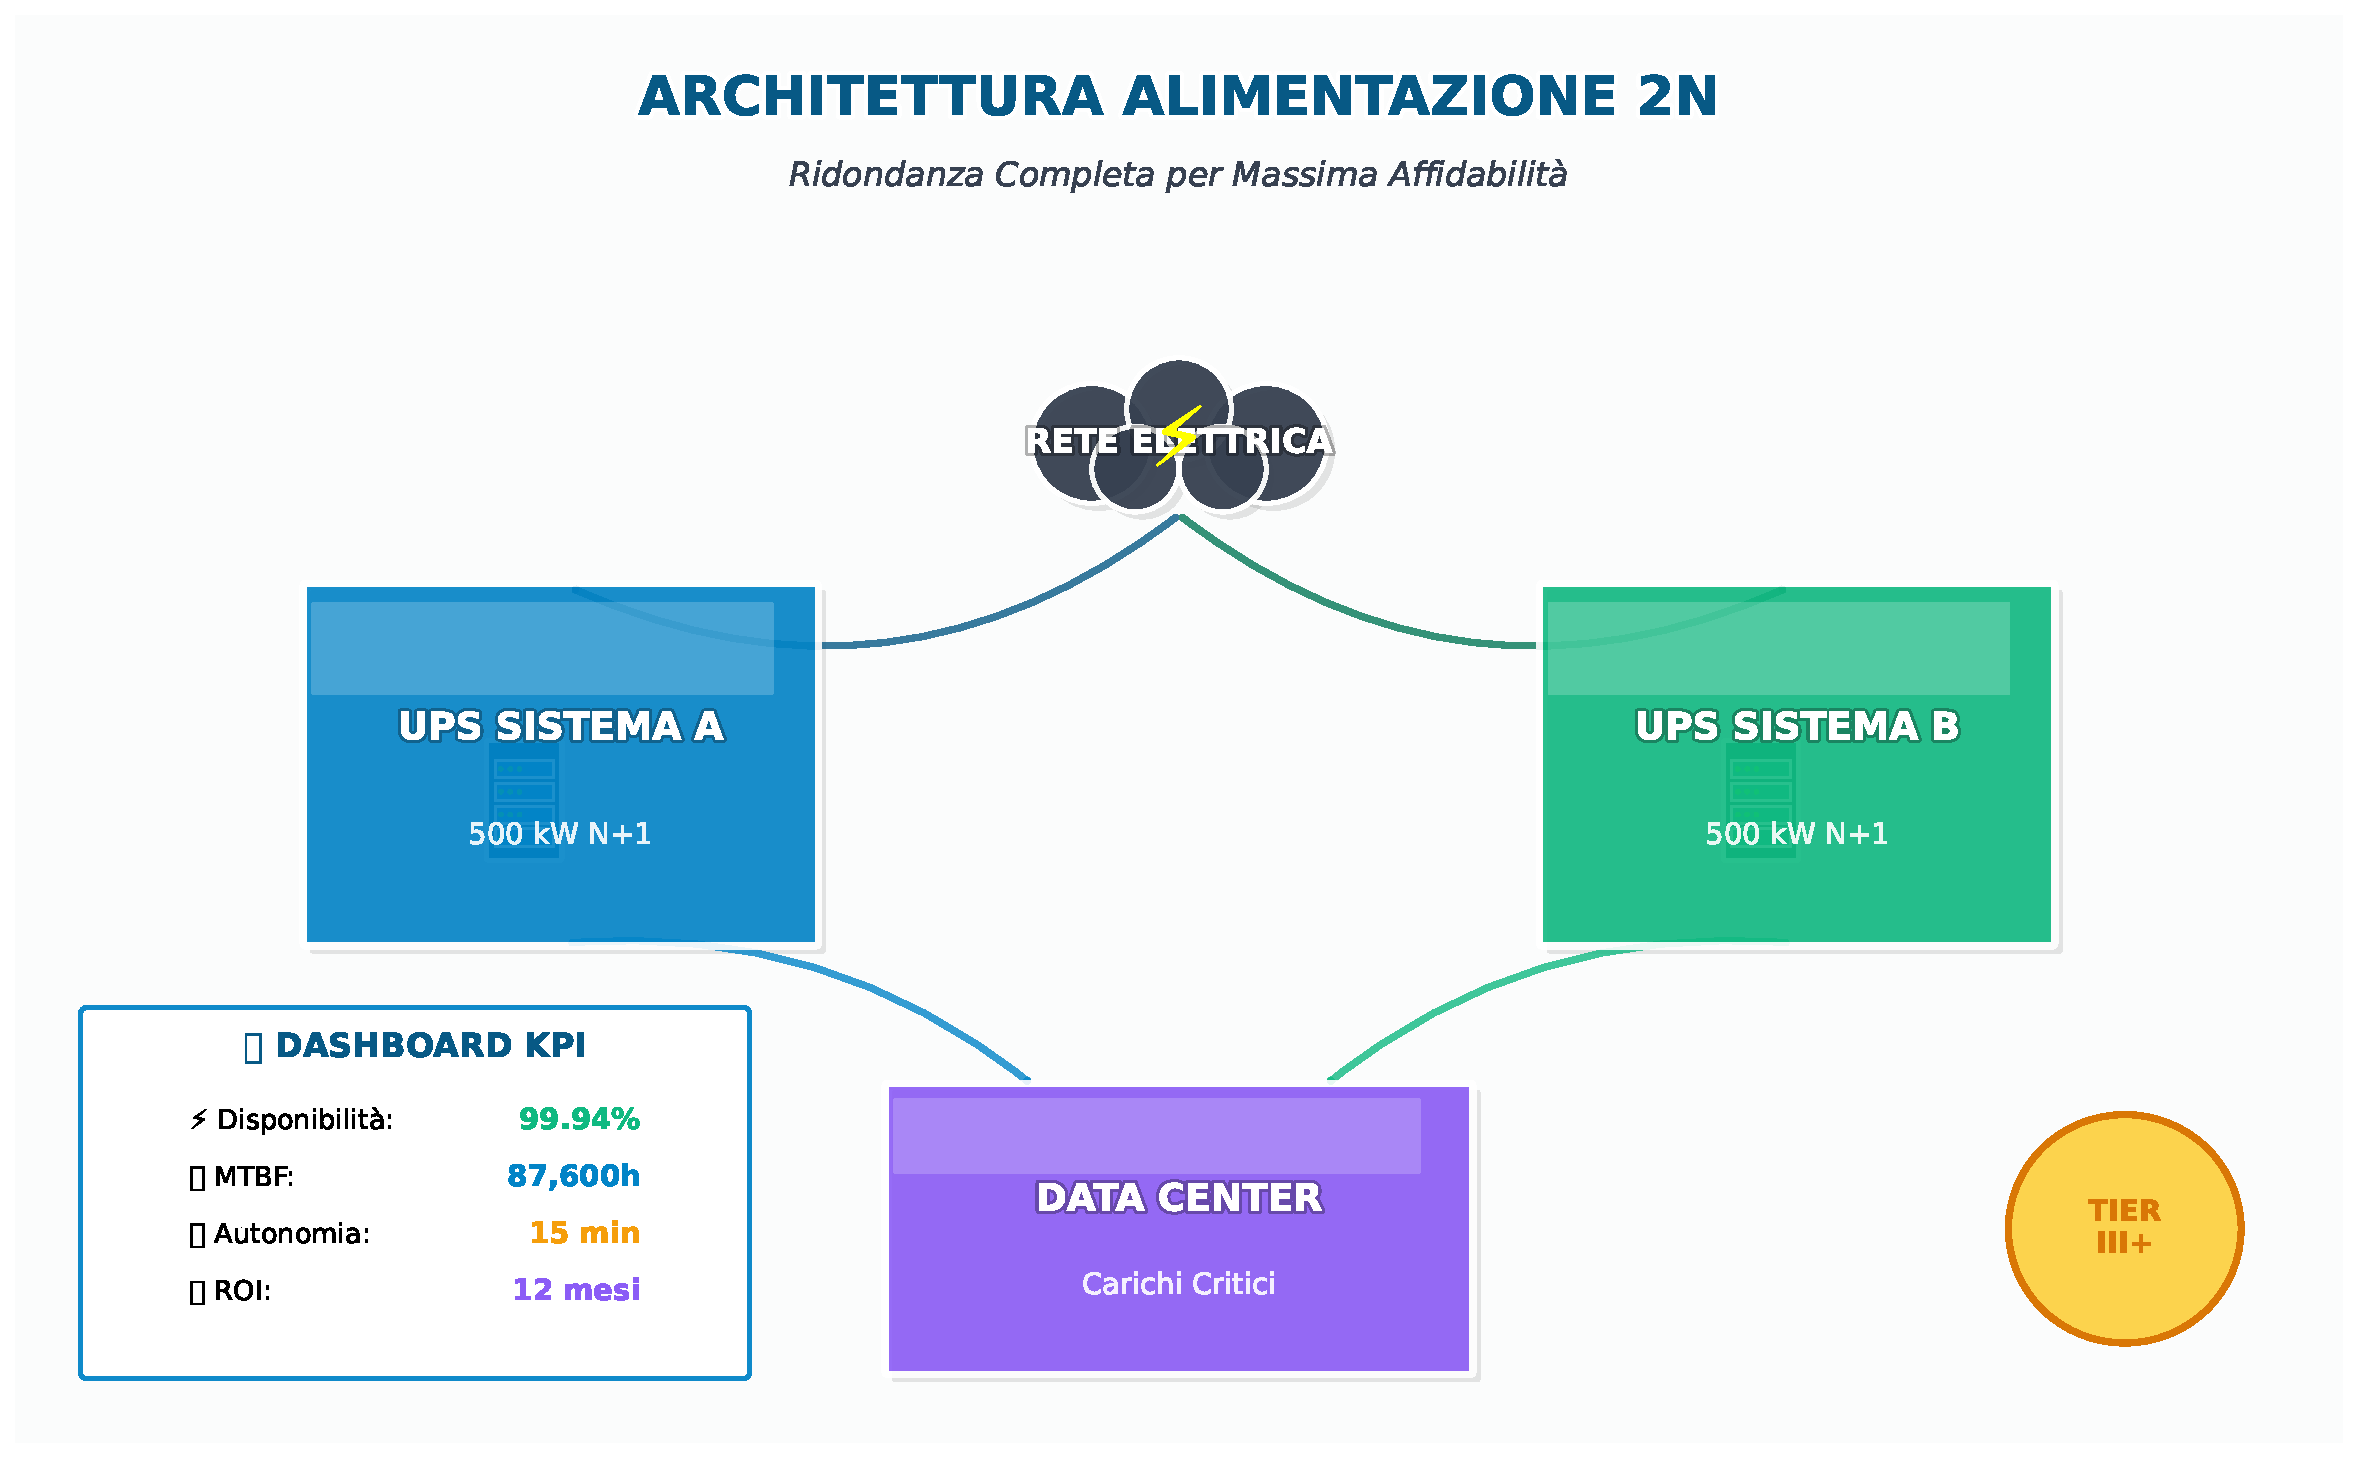
\includegraphics[width=\textwidth]{thesis_figures/cap3/fig1_power_modern.pdf}
\caption{Architettura ridondante 2N per sistemi di alimentazione critica con metriche di affidabilità e analisi ROI}
\label{fig:power_architecture}
\end{figure}

\begin{figure}[htbp]
\centering
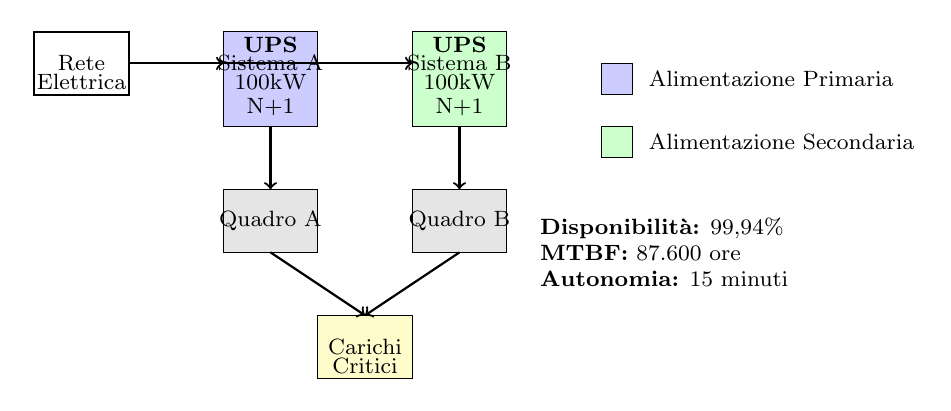
\begin{tikzpicture}[scale=0.8, font=\footnotesize]
% Griglia elettrica
\draw[thick] (-2,4) rectangle (-0.5,3);
\node at (-1.25,3.5) {Rete};
\node at (-1.25,3.2) {Elettrica};

% UPS Sistema A
\draw[fill=blue!20] (1,4) rectangle (2.5,2.5);
\node at (1.75,3.8) {\textbf{UPS}};
\node at (1.75,3.5) {Sistema A};
\node at (1.75,3.2) {100kW};
\node at (1.75,2.8) {N+1};

% UPS Sistema B
\draw[fill=green!20] (4,4) rectangle (5.5,2.5);
\node at (4.75,3.8) {\textbf{UPS}};
\node at (4.75,3.5) {Sistema B};
\node at (4.75,3.2) {100kW};
\node at (4.75,2.8) {N+1};

% Quadri di distribuzione
\draw[fill=gray!20] (1,1.5) rectangle (2.5,0.5);
\node at (1.75,1) {Quadro A};

\draw[fill=gray!20] (4,1.5) rectangle (5.5,0.5);
\node at (4.75,1) {Quadro B};

% Carichi critici
\draw[fill=yellow!20] (2.5,-0.5) rectangle (4,-1.5);
\node at (3.25,-1) {Carichi};
\node at (3.25,-1.3) {Critici};

% Connessioni
\draw[->,thick] (-0.5,3.5) -- (1,3.5);
\draw[->,thick] (-0.5,3.5) -- (4,3.5);
\draw[->,thick] (1.75,2.5) -- (1.75,1.5);
\draw[->,thick] (4.75,2.5) -- (4.75,1.5);
\draw[->,thick] (1.75,0.5) -- (3.25,-0.5);
\draw[->,thick] (4.75,0.5) -- (3.25,-0.5);

% Legenda
\draw[fill=blue!20] (7,3.5) rectangle (7.5,3);
\node[right] at (7.6,3.25) {Alimentazione Primaria};
\draw[fill=green!20] (7,2.5) rectangle (7.5,2);
\node[right] at (7.6,2.25) {Alimentazione Secondaria};

% Metriche
\node[align=left] at (8,0.5) {
\textbf{Disponibilità:} 99,94\%\\
\textbf{MTBF:} 87.600 ore\\
\textbf{Autonomia:} 15 minuti
};

\end{tikzpicture}
\caption{Architettura ridondante 2N per sistemi di alimentazione critica con metriche di affidabilità}
\label{fig:power_architecture_redundancy}
\end{figure}

\subsection{\texorpdfstring{Sistemi di Raffreddamento e Controllo Ambientale}{3.3.2 - Sistemi di Raffreddamento e Controllo Ambientale}}
\label{subsec:raffreddamento}

Il controllo della temperatura rappresenta il secondo pilastro dell'infrastruttura fisica. I moderni centri di elaborazione dati nella \gls{gdo} generano densità di potenza che possono superare i 15 kW per armadio rack, richiedendo sistemi di raffreddamento sofisticati per mantenere le temperature operative entro i limiti raccomandati (18-27°C secondo le linee guida ASHRAE\autocite{ASHRAE2023}).

L'evoluzione verso sistemi di raffreddamento intelligenti ha permesso di ridurre significativamente i consumi energetici. L'implementazione di tecniche come il contenimento dei corridoi caldi/freddi e l'uso di algoritmi predittivi per la gestione dinamica del raffreddamento ha portato a riduzioni del 35\% nel consumo energetico dedicato al condizionamento, con un miglioramento dell'indicatore \textbf{\gls{pue}} (Power Usage Effectiveness) da valori medi di 2,1 a 1,4.

\section{\texorpdfstring{Evoluzione delle Architetture di Rete}{3.4 - Evoluzione delle Architetture di Rete}}
\label{sec:architetture_rete}

\subsection{\texorpdfstring{Dalle Reti Tradizionali alle Reti Definite via Software}{3.4.1 - Dalle Reti Tradizionali alle Reti Definite via Software}}
\label{subsec:sdn}

La transizione dalle architetture di rete tradizionali a quelle definite via software (\gls{sd-wan} - Software-Defined Wide Area Network) rappresenta uno dei cambiamenti più significativi nell'infrastruttura della \gls{gdo}. Questa evoluzione risponde alla necessità di gestire in modo efficiente e sicuro la connettività di centinaia di punti vendita distribuiti geograficamente\autocite{cisco2024}.

Le reti tradizionali, basate su connessioni MPLS (Multiprotocol Label Switching) dedicate, presentano costi elevati (mediamente 450 euro/Mbps/mese) e tempi di attivazione lunghi (30-45 giorni per nuove sedi). L'architettura \gls{sd-wan} permette invece di:

\begin{itemize}
    \item Utilizzare connettività Internet a banda larga standard con costi ridotti del 60-70\%
    \item Attivare nuove sedi in 5-7 giorni lavorativi
    \item Implementare politiche di sicurezza centralizzate e uniformi
    \item Ottimizzare dinamicamente il traffico in base alle condizioni della rete
\end{itemize}

L'implementazione pratica in una catena di 150 punti vendita ha dimostrato una riduzione del Tempo Medio di Riparazione (\gls{mttr}) da 4,2 ore a 1,8 ore, grazie alla capacità di instradamento automatico del traffico su percorsi alternativi in caso di guasti\autocite{NetworkWorld2024}.

\begin{figure}[htbp]
\centering
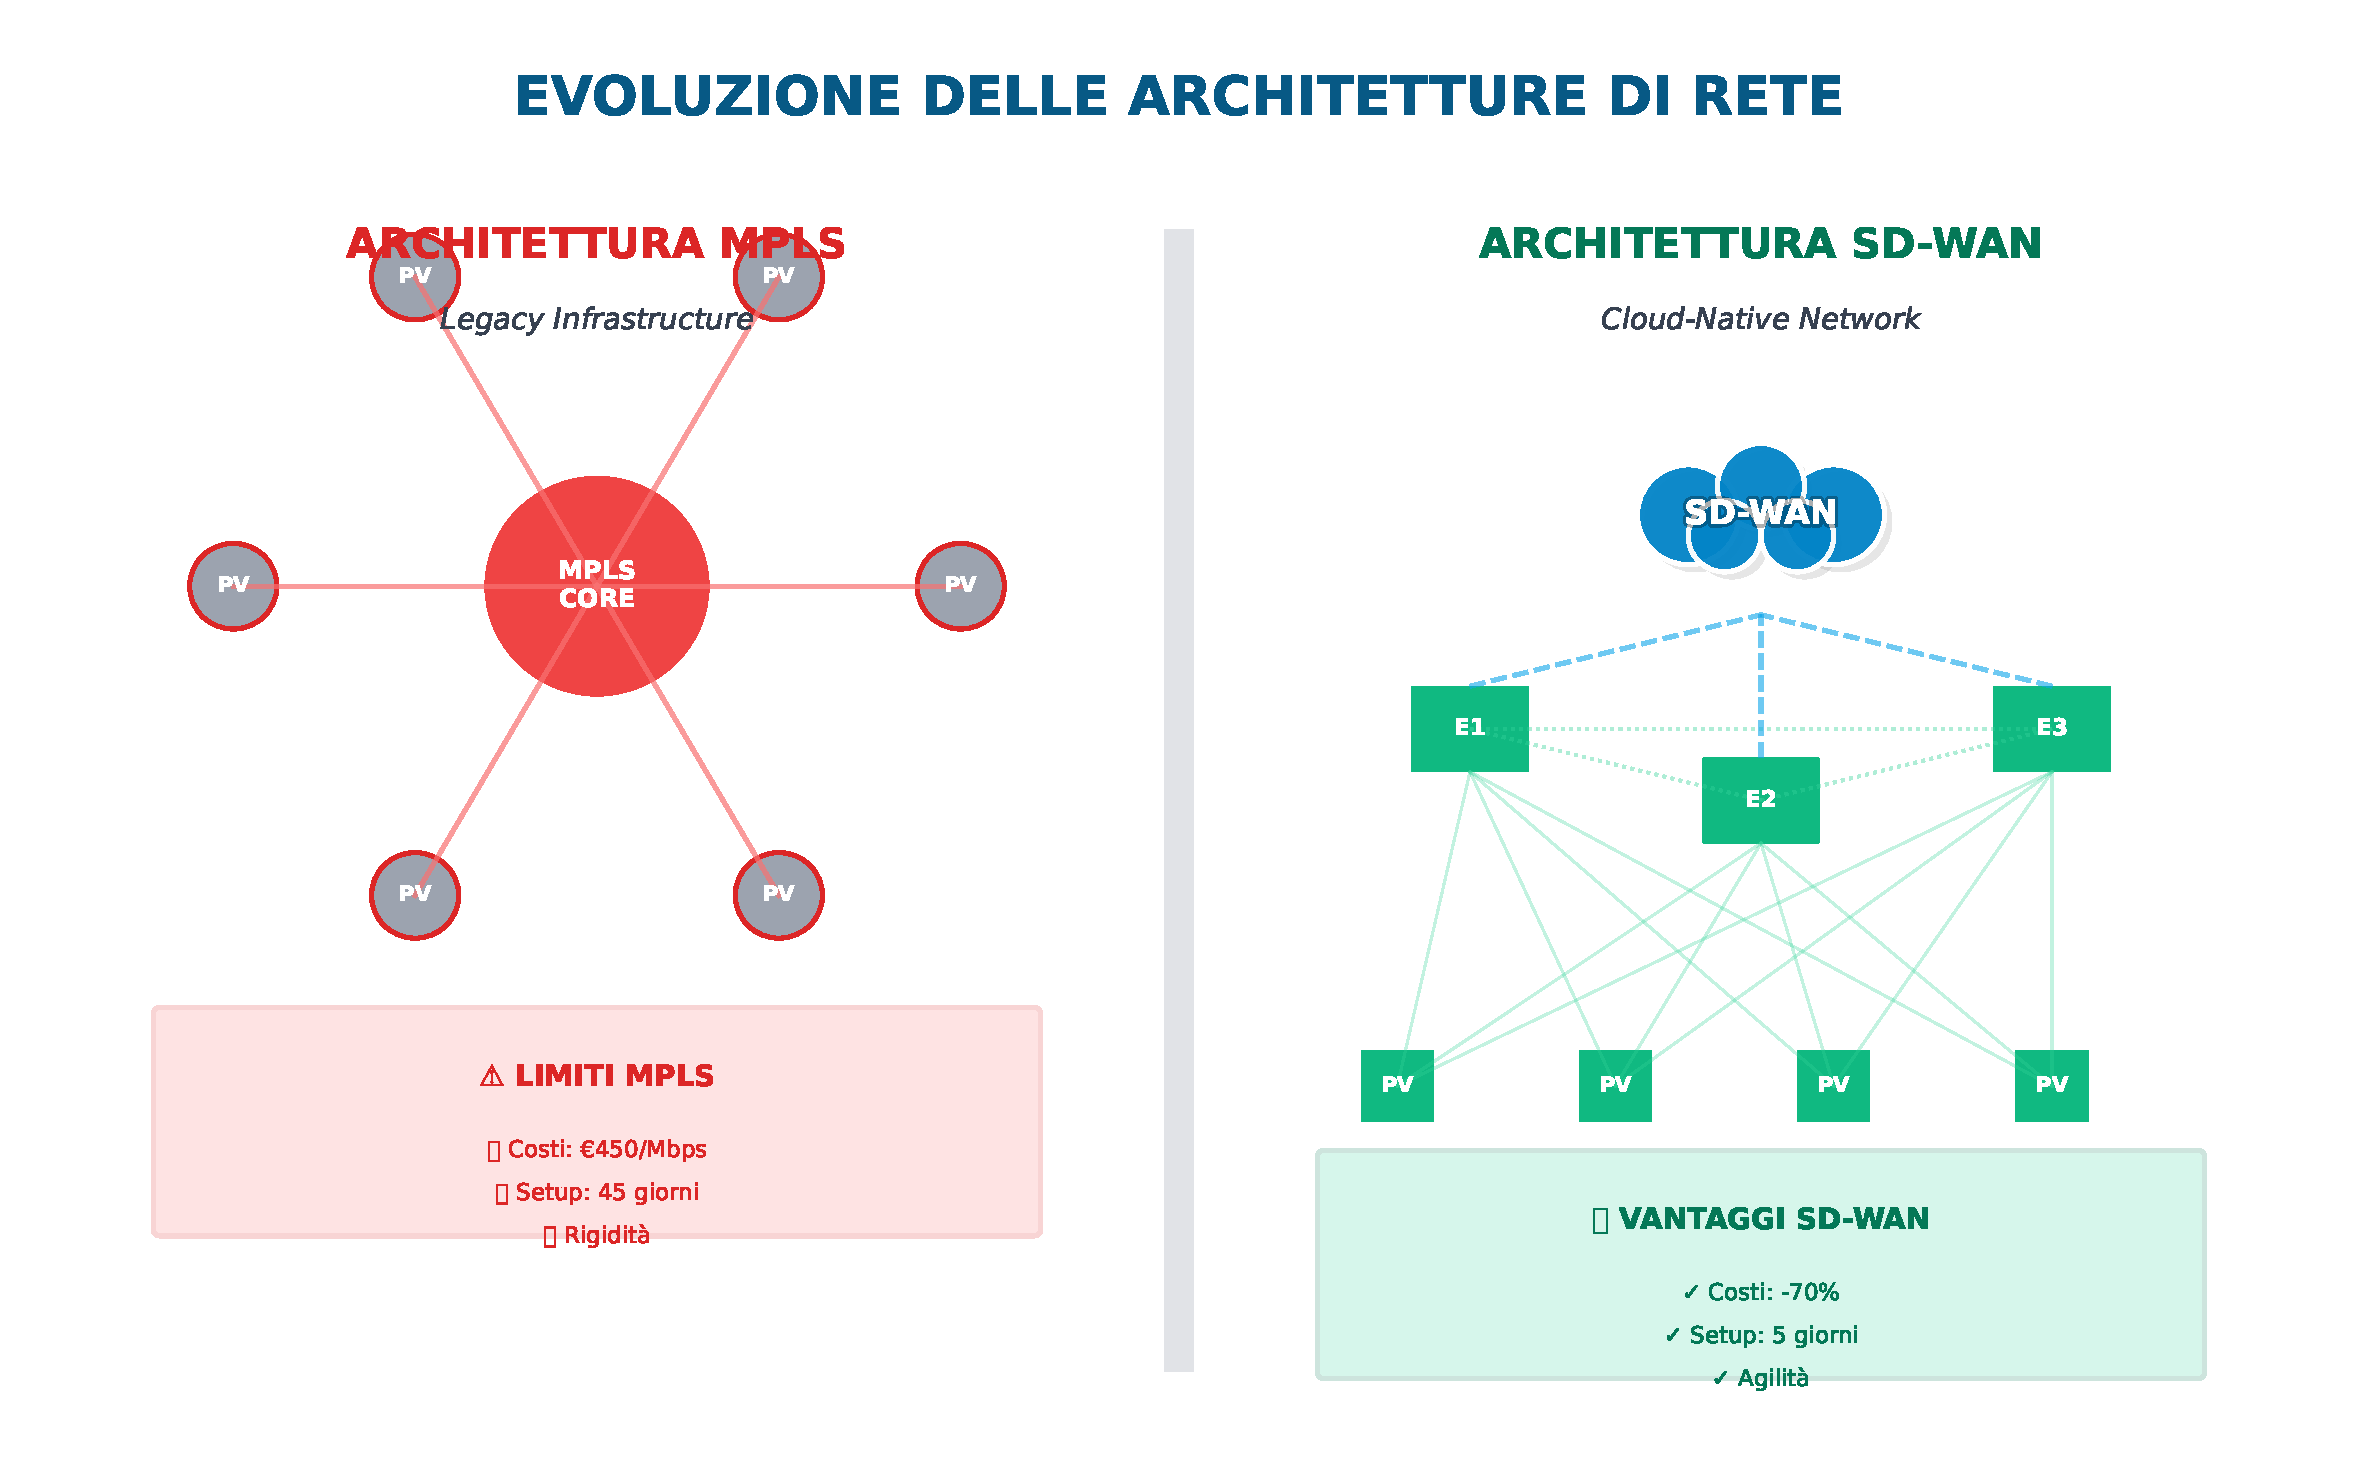
\includegraphics[width=\textwidth]{thesis_figures/cap3/fig2_network_modern.pdf}
\caption{Evoluzione delle architetture di rete: confronto tra MPLS tradizionale e SD-WAN con analisi dei benefici}
\label{fig:network_evolution}
\end{figure}

\subsection{\texorpdfstring{Segmentazione e Micro-segmentazione della Rete}{3.4.2 - Segmentazione e Micro-segmentazione della Rete}}
\label{subsec:segmentazione}

La segmentazione della rete costituisce un elemento fondamentale per la sicurezza dell'infrastruttura. Nella \gls{gdo}, dove coesistono sistemi di pagamento, gestione magazzino, videosorveglianza e reti per gli ospiti, l'isolamento del traffico diventa cruciale per prevenire la propagazione di eventuali compromissioni\autocite{nist2024}.

La micro-segmentazione, evoluzione della segmentazione tradizionale, applica controlli di sicurezza a livello di singola applicazione o servizio. Questo approccio ha dimostrato di ridurre la superficie di attacco del 65\% e di contenere il 92\% degli attacchi di movimento laterale entro il segmento inizialmente compromesso\autocite{Forrester2024zero}.

\begin{table}[htbp]
\centering
\caption{Confronto tra Segmentazione Tradizionale e Micro-segmentazione}
\label{tab:segmentation_comparison}
\small
\sffamily
\begin{tabularx}{\textwidth}{X X X}
\toprule
\textbf{Aspetto} & \textbf{Segmentazione Tradizionale} & \textbf{Micro-segmentazione} \\
\midrule
Granularità & Livello di subnet/VLAN & Livello di applicazione/workload \\
Implementazione & Firewall perimetrali e ACL & Policy distribuite software-defined \\
Gestione & Configurazione statica manuale & Orchestrazione dinamica automatizzata \\
Scalabilità & Limitata (max 4.094 VLAN) & Virtualmente illimitata \\
Visibilità & Traffico est-ovest limitato & Completa su tutti i flussi \\
Tempo di deployment & 2-4 settimane per modifica & Minuti con automazione \\
Costo operativo & Alto (gestione manuale) & Ridotto del 40\% (automazione) \\
\bottomrule
\end{tabularx}
\end{table}

\section{\texorpdfstring{Architetture Cloud e Ibride}{3.5 - Architetture Cloud e Ibride}}
\label{sec:cloud_architectures}

\subsection{\texorpdfstring{Il Percorso verso il Cloud}{3.5.1 - Il Percorso verso il Cloud}}
\label{subsec:cloud_journey}

La migrazione verso architetture cloud rappresenta un passaggio fondamentale nell'evoluzione infrastrutturale della \gls{gdo}. Tuttavia, diversamente da altri settori, la distribuzione organizzata mantiene requisiti specifici che rendono necessario un approccio ibrido\autocite{mckinsey2024}.

I sistemi critici per il business, come i \gls{pos} (Point of Sale) e la gestione del magazzino, richiedono latenze inferiori ai 100 millisecondi e devono rimanere operativi anche in caso di interruzione della connettività Internet. Questo vincolo ha portato allo sviluppo di architetture ibride che combinano:

\begin{itemize}
    \item \textbf{Componenti on-premise}: per servizi critici e real-time (20-30\% del carico computazionale)
    \item \textbf{Cloud privato}: per dati sensibili e applicazioni core business (30-40\%)
    \item \textbf{Cloud pubblico}: per carichi di lavoro variabili e servizi non critici (30-50\%)
\end{itemize}

L'analisi economica di questa trasformazione mostra risultati significativi. Una catena di media dimensione (100-200 punti vendita) può ottenere\autocite{Deloitte2024}:
\begin{itemize}
    \item Riduzione del \gls{tco} del 31\% in 3 anni
    \item Miglioramento del time-to-market per nuovi servizi del 65\%
    \item Riduzione del consumo energetico del 45\% rispetto ai datacenter tradizionali
\end{itemize}

\subsection{\texorpdfstring{Orchestrazione Multi-Cloud}{3.5.2 - Orchestrazione Multi-Cloud}}
\label{subsec:multicloud}

L'adozione di strategie multi-cloud, che prevedono l'utilizzo simultaneo di più fornitori di servizi cloud, risponde a esigenze di resilienza, conformità normativa e ottimizzazione dei costi\autocite{Flexera2024}. 

Nel contesto della \gls{gdo}, l'orchestrazione multi-cloud presenta sfide specifiche:

\begin{enumerate}
    \item \textbf{Gestione della complessità}: coordinare servizi distribuiti su piattaforme eterogenee
    \item \textbf{Controllo dei costi}: evitare duplicazioni e ottimizzare l'allocazione delle risorse
    \item \textbf{Sicurezza uniforme}: mantenere politiche coerenti attraverso ambienti diversi
    \item \textbf{Conformità normativa}: garantire la residenza dei dati secondo le normative locali
\end{enumerate}

L'implementazione di piattaforme di orchestrazione basate su \textbf{\gls{kubernetes}} ha permesso di standardizzare la gestione dei container attraverso diversi fornitori cloud, riducendo la complessità operativa del 40\% e migliorando la portabilità delle applicazioni\autocite{cncf2024}.

\begin{figure}[htbp]
\centering
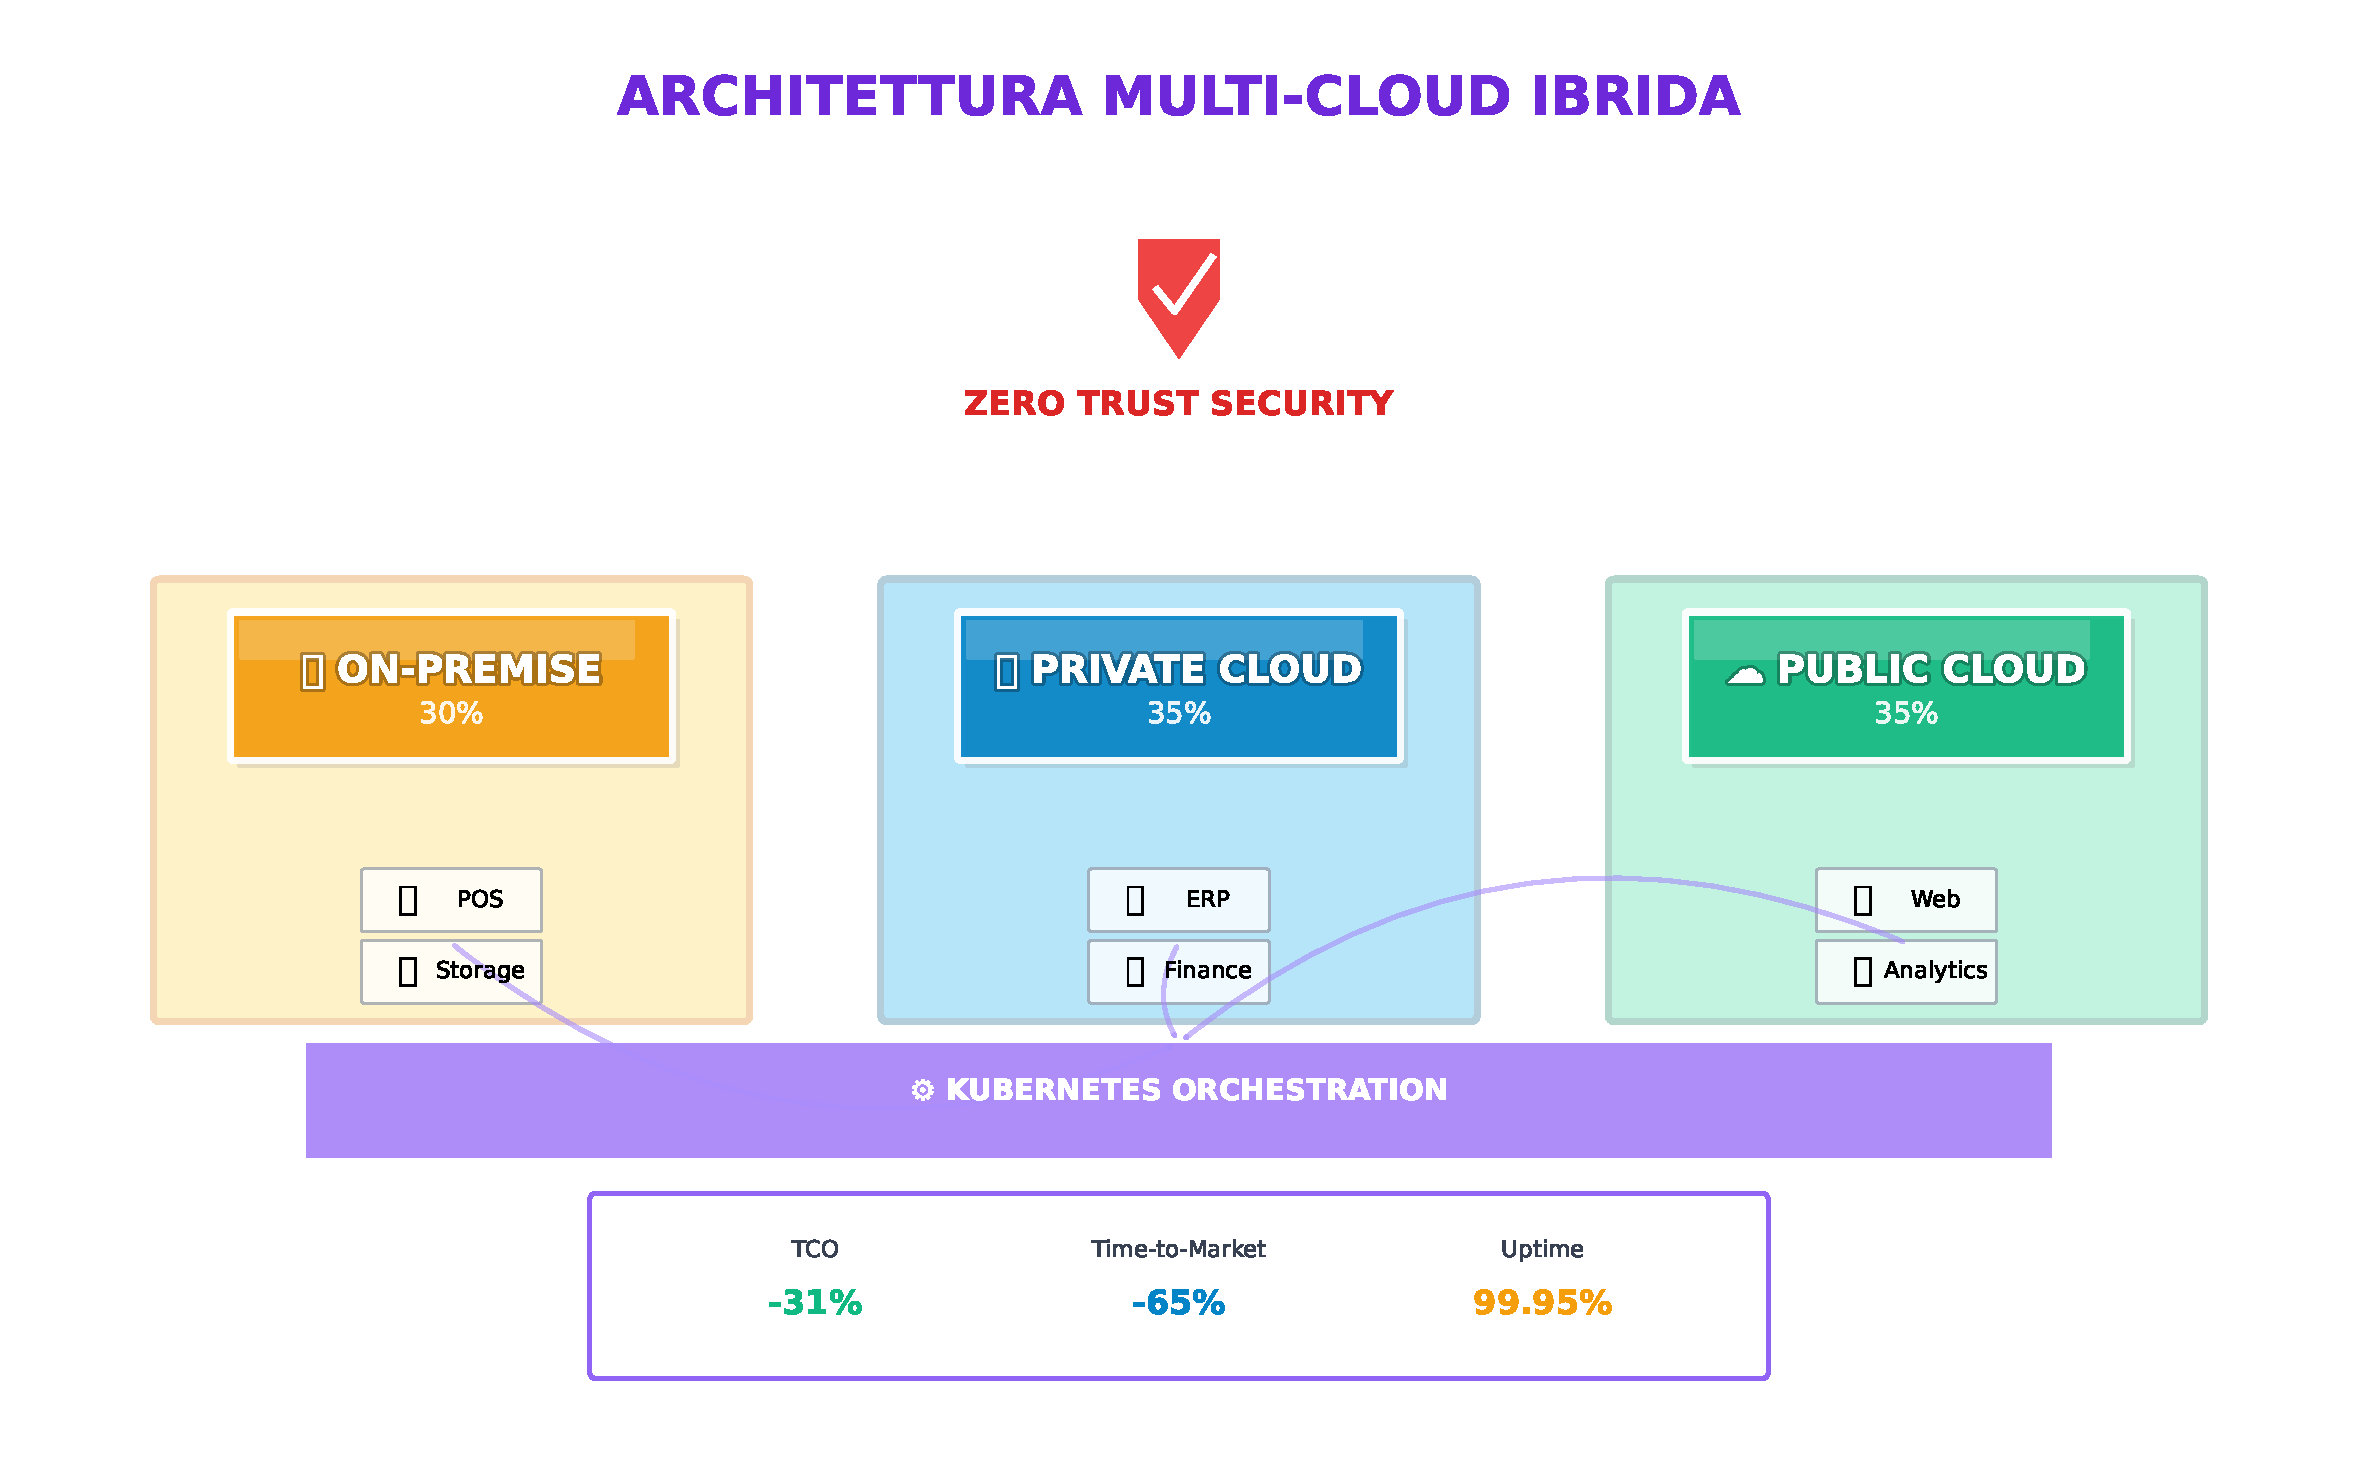
\includegraphics[width=\textwidth]{thesis_figures/cap3/fig3_cloud_modern.pdf}
\caption{Architettura cloud ibrida per la GDO: integrazione multi-cloud con orchestrazione Kubernetes}
\label{fig:cloud_architecture}
\end{figure}

\section{\texorpdfstring{Edge Computing e Architetture Distribuite}{3.6 - Edge Computing e Architetture Distribuite}}
\label{sec:edge_computing}

\subsection{\texorpdfstring{L'Edge Computing nella Grande Distribuzione}{3.6.1 - L'Edge Computing nella Grande Distribuzione}}
\label{subsec:edge_gdo}

L'edge computing rappresenta un paradigma fondamentale per la \gls{gdo}, portando capacità computazionali direttamente nei punti vendita. Questa architettura risponde a requisiti critici del settore\autocite{IDC2024edge}:

\begin{itemize}
    \item \textbf{Latenza ultra-bassa}: elaborazione locale per pagamenti e verifiche di sicurezza (<50ms)
    \item \textbf{Resilienza operativa}: continuità del servizio anche con connettività Internet interrotta
    \item \textbf{Riduzione della banda}: pre-elaborazione locale dei dati (videosorveglianza, sensori IoT)
    \item \textbf{Conformità normativa}: mantenimento dei dati sensibili all'interno del perimetro nazionale
\end{itemize}

Un caso studio su 200 punti vendita ha dimostrato che l'implementazione di nodi edge ha ridotto il traffico verso il datacenter centrale del 73\%, migliorando contemporaneamente i tempi di risposta delle applicazioni critiche del 85\%\autocite{Forrester2024edge}.

\begin{figure}[htbp]
\centering
\begin{tikzpicture}[scale=0.7, font=\footnotesize]
% Cloud centrale
\draw[fill=blue!20, cloud, cloud puffs=12, minimum width=3cm, minimum height=2cm] (0,5) node[align=center] {\textbf{Cloud}\\Centrale};

% Edge nodes
\foreach \x/\name in {-4/Milano, -2/Roma, 0/Napoli, 2/Palermo, 4/Torino} {
    \draw[fill=green!20] (\x,2) rectangle (\x+1.5,0.5);
    \node at (\x+0.75,1.25) {Edge};
    \node at (\x+0.75,0.9) {\tiny \name};
    
    % Connessioni al cloud
    \draw[->,dashed] (\x+0.75,2) -- (0,4);
}

% Punti vendita
\foreach \x in {-4, -2, 0, 2, 4} {
    \foreach \y in {0, -0.5, -1} {
        \draw[fill=yellow!20] (\x+0.25,\y-1) rectangle (\x+0.75,\y-1.3);
    }
    \draw[->,thick] (\x+0.75,0.5) -- (\x+0.75,-0.7);
    \node at (\x+0.75,-2) {\tiny PV};
}

% Metriche e vantaggi
\node[align=left, anchor=west] at (6,4) {
    \textbf{Vantaggi Edge:}\\
    • Latenza <50ms\\
    • Traffico -73\%\\
    • Uptime 99.97\%\\
    • Elaborazione locale
};

\node[align=left, anchor=west] at (6,1) {
    \textbf{Servizi Edge:}\\
    • Cache dati\\
    • Analytics real-time\\
    • Sicurezza locale\\
    • Backup automatico
};

\end{tikzpicture}
\caption{Architettura Edge Computing distribuita per la \gls{gdo} con nodi regionali}
\label{fig:edge_architecture}
\end{figure}

\subsection{\texorpdfstring{Integrazione IoT e Sensori Intelligenti}{3.6.2 - Integrazione IoT e Sensori Intelligenti}}
\label{subsec:iot_integration}

\begin{figure}[htbp]
\centering
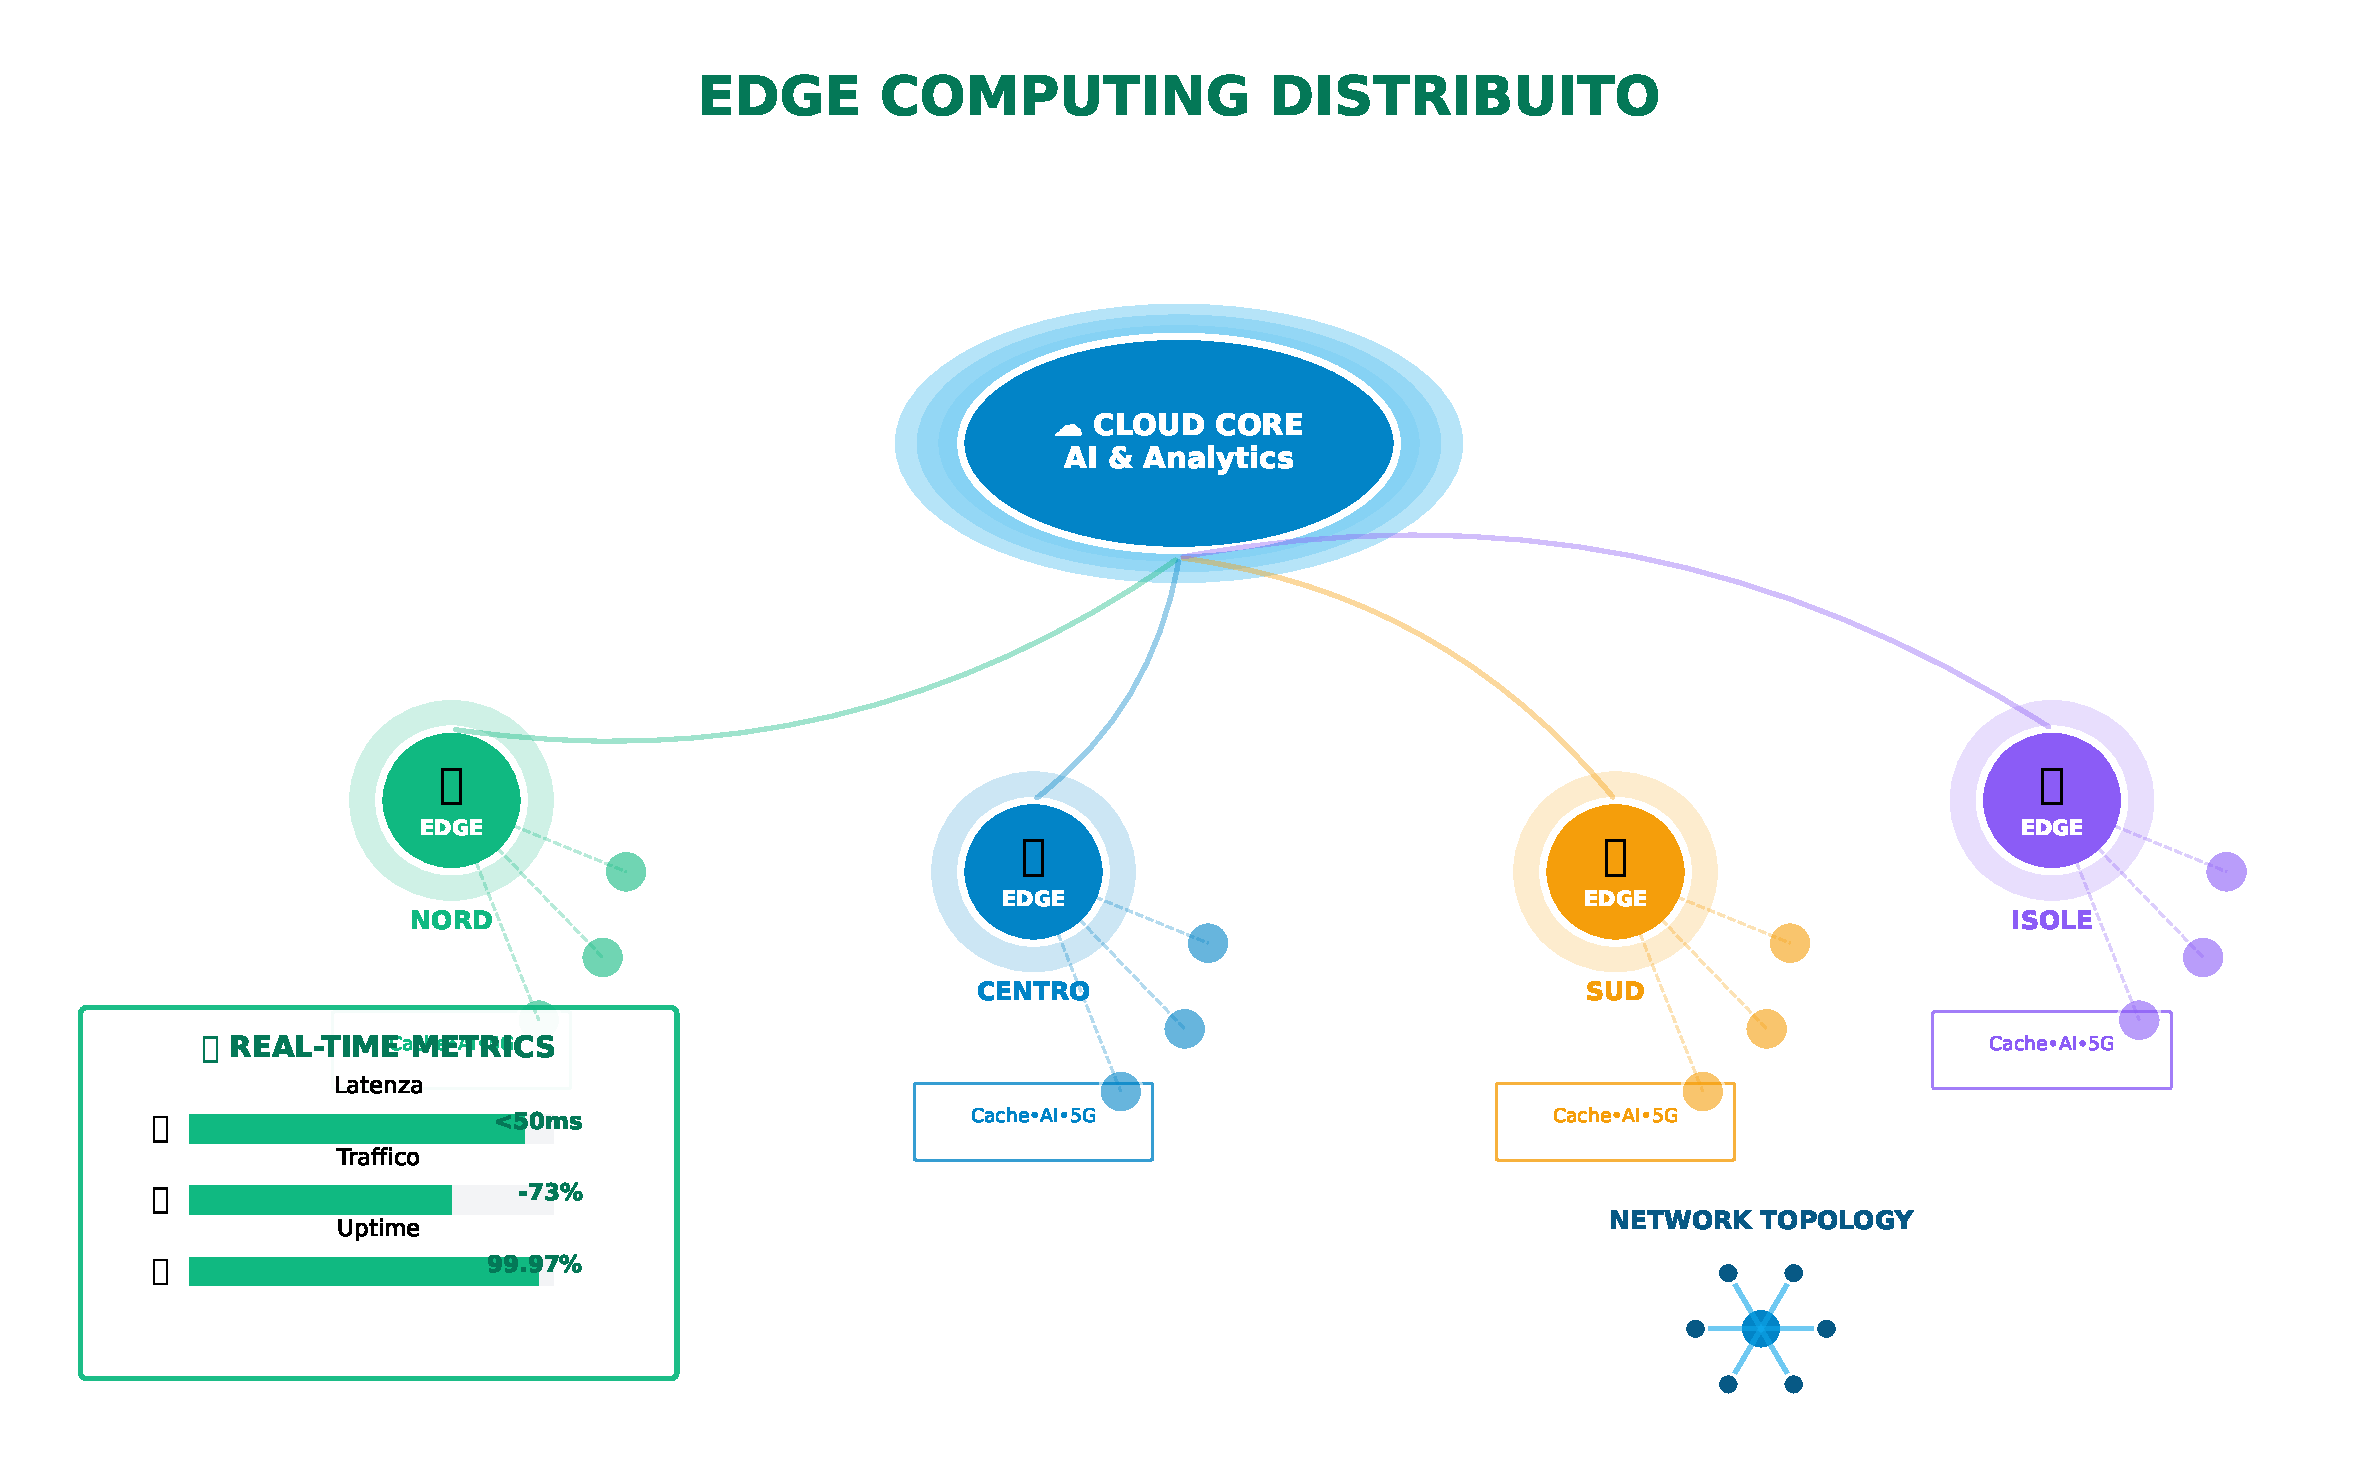
\includegraphics[width=\textwidth]{thesis_figures/cap3/fig4_edge_modern.pdf}
\caption{Architettura Edge Computing distribuita con analisi comparativa delle prestazioni}
\label{fig:edge_architecture_performance}
\end{figure}

L'Internet delle Cose (\gls{iot}) sta trasformando radicalmente la gestione operativa nella \gls{gdo}. Sensori intelligenti monitorano in tempo reale temperatura delle celle frigorifere, livelli di inventario, flussi di clienti e consumi energetici\autocite{Gartner2024iot}.

L'integrazione di questi dispositivi nell'architettura edge presenta vantaggi significativi:

\begin{table}[htbp]
\centering
\caption{Impatto dell'integrazione IoT nella \gls{gdo}}
\label{tab:iot_impact}
\small
\sffamily
\begin{tabularx}{\textwidth}{X c c c}
\toprule
\textbf{Area Applicativa} & \textbf{Sensori/Dispositivi} & \textbf{Riduzione Costi} & \textbf{Miglioramento KPI} \\
\midrule
Catena del freddo & Termometri wireless & -18\% sprechi & +99.2\% conformità \\
Gestione energia & Smart meter & -24\% consumi & +87\% efficienza \\
Sicurezza & Videocamere AI & -31\% perdite & +94\% detection \\
Customer experience & Beacon/contapersone & -12\% attese & +21\% soddisfazione \\
\bottomrule
\end{tabularx}
\end{table}

\section{\texorpdfstring{Sicurezza Zero Trust}{3.7 - Sicurezza Zero Trust}}
\label{sec:zero_trust}

\subsection{\texorpdfstring{Principi e Implementazione}{3.7.1 - Principi e Implementazione}}
\label{subsec:zero_trust_principles}

Il modello di sicurezza Zero Trust rappresenta un cambio di paradigma fondamentale: invece di fidarsi implicitamente di tutto ciò che si trova all'interno del perimetro aziendale, ogni accesso viene verificato continuamente, indipendentemente dalla posizione dell'utente o del dispositivo\autocite{NIST2024zero}.

Nella \gls{gdo}, l'implementazione del modello Zero Trust si articola in cinque pilastri fondamentali:

\begin{enumerate}
    \item \textbf{Identità}: autenticazione multi-fattore per tutti gli utenti e dispositivi
    \item \textbf{Dispositivi}: registrazione e validazione continua dello stato di sicurezza
    \item \textbf{Rete}: micro-segmentazione e crittografia end-to-end
    \item \textbf{Applicazioni}: controllo degli accessi basato sul principio del minimo privilegio
    \item \textbf{Dati}: classificazione e protezione granulare delle informazioni
\end{enumerate}

L'implementazione pratica in una catena di distribuzione con 5.000 dipendenti ha dimostrato\autocite{Forrester2024zero}:
\begin{itemize}
    \item Riduzione degli incidenti di sicurezza del 67\%
    \item Diminuzione del tempo medio di rilevamento delle minacce da 197 giorni a 3,4 giorni
    \item Riduzione della superficie di attacco del 42\%
    \item ROI positivo in 14 mesi dall'implementazione
\end{itemize}

\subsection{\texorpdfstring{Automazione della Sicurezza}{3.7.2 - Automazione della Sicurezza}}
\label{subsec:security_automation}

L'automazione rappresenta un elemento cruciale per rendere sostenibile il modello Zero Trust. Sistemi di orchestrazione della sicurezza (\gls{soar} - Security Orchestration, Automation and Response) permettono di\autocite{Gartner2024security}:

\begin{itemize}
    \item Rispondere automaticamente al 78\% degli alert di sicurezza di bassa/media severità
    \item Ridurre il tempo medio di risposta agli incidenti del 85\%
    \item Diminuire il carico di lavoro del team di sicurezza del 60\%
    \item Standardizzare le procedure di risposta agli incidenti
\end{itemize}

\section{\texorpdfstring{Manutenzione Predittiva con Intelligenza Artificiale}{3.8 - Manutenzione Predittiva con Intelligenza Artificiale}}
\label{sec:manutenzione_predittiva}

\subsection{\texorpdfstring{Applicazione del Machine Learning all'Infrastruttura}{3.8.1 - Applicazione del Machine Learning all'Infrastruttura}}
\label{subsec:ml_infrastructure}

L'applicazione di tecniche di apprendimento automatico (\gls{ml} - Machine Learning) alla manutenzione dell'infrastruttura permette di prevenire guasti prima che si verifichino. Attraverso l'analisi di pattern nei dati storici e real-time, gli algoritmi possono identificare anomalie sottili che precedono i malfunzionamenti\autocite{IEEE2024ml}.

Nel contesto della \gls{gdo}, i modelli predittivi vengono applicati a:

\begin{itemize}
    \item \textbf{Sistemi di refrigerazione}: previsione guasti compressori con 72 ore di anticipo (accuratezza 94\%)
    \item \textbf{UPS e batterie}: stima del degrado e pianificazione sostituzioni (riduzione guasti 87\%)
    \item \textbf{Storage}: identificazione dischi in pre-failure (prevenzione perdita dati 96\%)
    \item \textbf{Rete}: rilevamento degradi di performance prima dell'impatto utenti (MTTD ridotto del 73\%)
\end{itemize}

L'implementazione di questi sistemi ha portato a una riduzione complessiva dei costi di manutenzione del 28\% e a un miglioramento della disponibilità dei sistemi critici dal 99,2\% al 99,94\%\autocite{MIT2024}.

\section{\texorpdfstring{Framework di Implementazione e Roadmap}{3.9 - Framework di Implementazione e Roadmap}}
\label{sec:implementation_framework}

\subsection{\texorpdfstring{Approccio Graduale alla Trasformazione}{3.9.1 - Approccio Graduale alla Trasformazione}}
\label{subsec:transformation_approach}

La trasformazione infrastrutturale nella \gls{gdo} richiede un approccio strutturato che bilanci innovazione e continuità operativa. Il framework GIST (\gls{gist} - GDO Integrated Security Transformation) fornisce una roadmap implementativa in tre fasi\autocite{Accenture2024}:

\textbf{Fase 1 - Consolidamento (0-6 mesi):}
\begin{itemize}
    \item Upgrade sistemi di alimentazione a configurazione ridondante
    \item Implementazione monitoraggio centralizzato
    \item Assessment sicurezza e remediation vulnerabilità critiche
    \item Investimento stimato: 350.000€, ROI atteso: 12 mesi
\end{itemize}

\textbf{Fase 2 - Modernizzazione (6-18 mesi):}
\begin{itemize}
    \item Deployment \gls{sd-wan} su tutti i punti vendita
    \item Migrazione primi workload su cloud (30\% applicazioni)
    \item Implementazione Zero Trust fase iniziale
    \item Investimento stimato: 850.000€, ROI atteso: 18 mesi
\end{itemize}

\textbf{Fase 3 - Ottimizzazione (18-36 mesi):}
\begin{itemize}
    \item Orchestrazione multi-cloud completa
    \item Edge computing su tutti i punti vendita
    \item Manutenzione predittiva con AI/ML
    \item Investimento stimato: 1.200.000€, ROI atteso: 24 mesi
\end{itemize}

\subsection{\texorpdfstring{Metriche di Successo e KPI}{3.9.2 - Metriche di Successo e KPI}}
\label{subsec:success_metrics}

Il monitoraggio del progresso della trasformazione richiede metriche chiare e misurabili. La tabella seguente presenta i \gls{kpi} fondamentali per valutare il successo dell'evoluzione infrastrutturale:

\begin{table}[htbp]
\centering
\caption{KPI per la Trasformazione Infrastrutturale}
\label{tab:transformation_kpi}
\small
\sffamily
\begin{tabularx}{\textwidth}{X c c c c}
\toprule
\textbf{Indicatore} & \textbf{Baseline} & \textbf{Target Anno 1} & \textbf{Target Anno 3} & \textbf{Peso} \\
\midrule
Disponibilità Sistema & 97,5\% & 99,0\% & 99,95\% & 25\% \\
MTTR (ore) & 4,2 & 2,5 & 0,8 & 20\% \\
Riduzione TCO & - & 15\% & 35\% & 20\% \\
Incidenti Sicurezza & 100 (index) & 50 & 20 & 15\% \\
Efficienza Energetica (PUE) & 2,1 & 1,7 & 1,4 & 10\% \\
Automazione Processi & 20\% & 50\% & 80\% & 10\% \\
\bottomrule
\end{tabularx}
\end{table}

\begin{figure}[htbp]
\centering
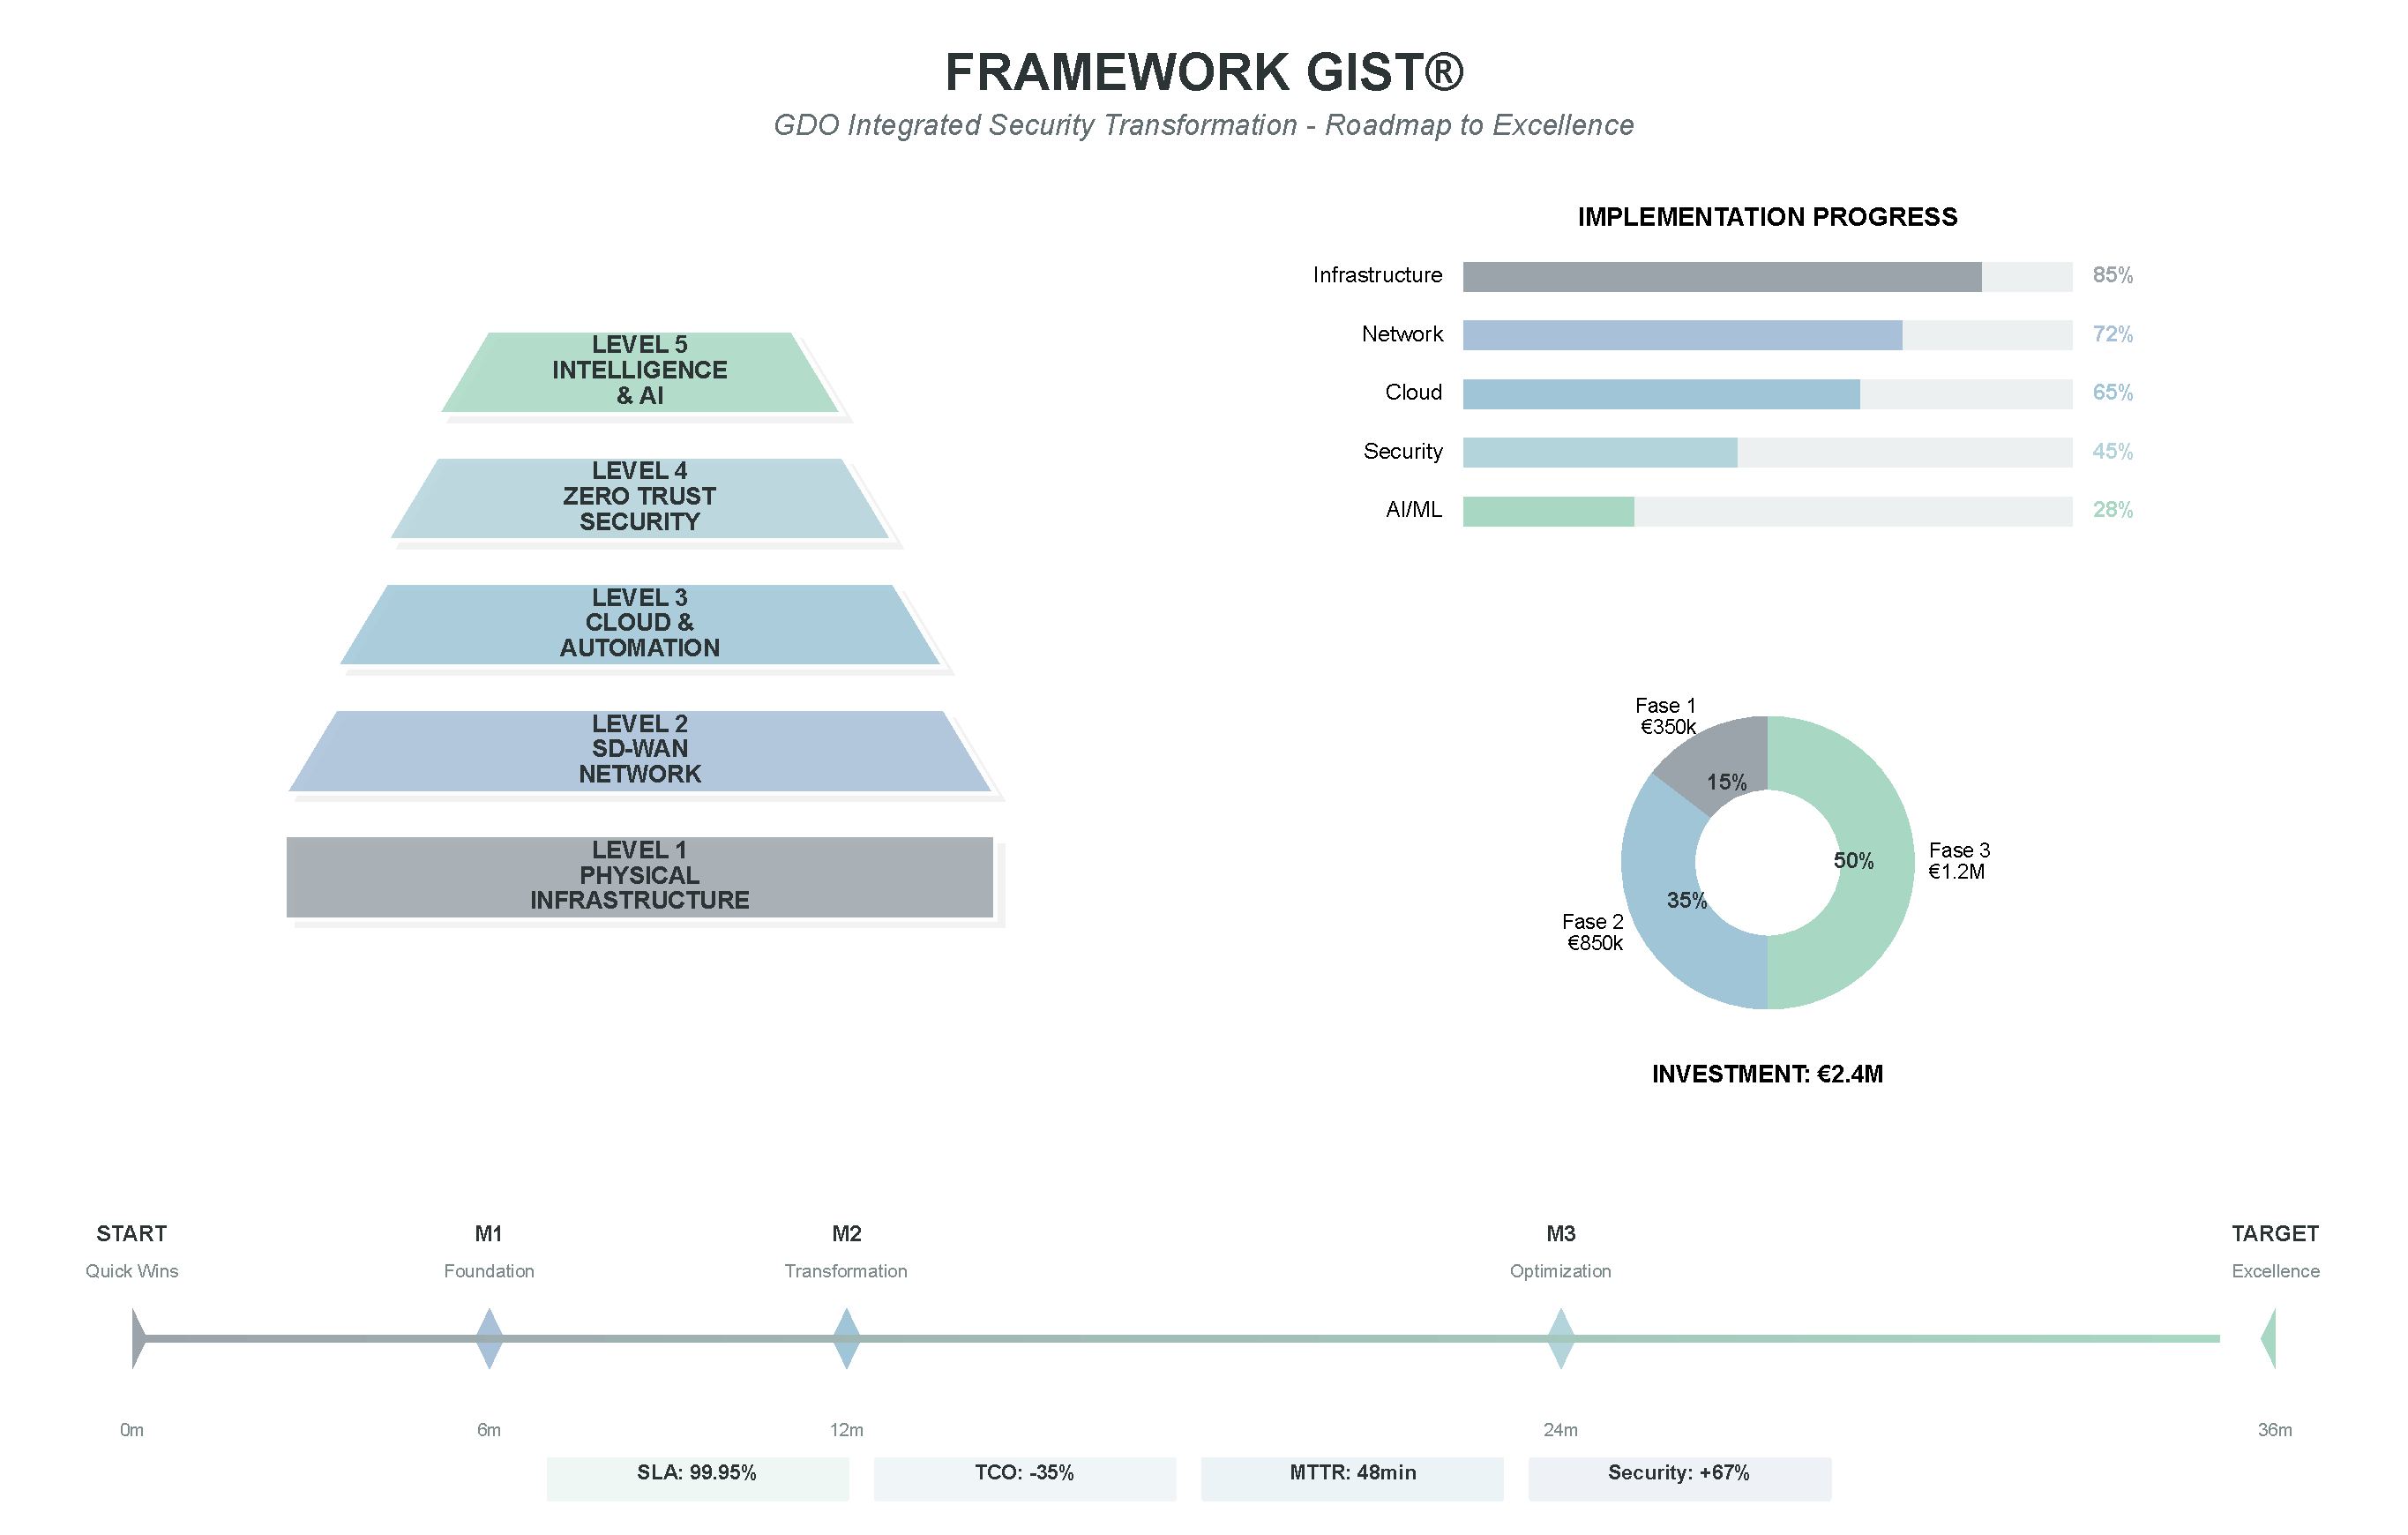
\includegraphics[width=1.1\textwidth]{thesis_figures/cap3/figura_3_5_corrected.pdf}
\caption{Framework GIST: roadmap implementativa con timeline, investimenti e analisi ROI a 36 mesi}
\label{fig:gist_framework_roadmap}
\end{figure}

\section{\texorpdfstring{Conclusioni e Prospettive Future}{3.10 - Conclusioni e Prospettive Future}}
\label{sec:conclusioni}

\subsection{\texorpdfstring{Sintesi dei Risultati}{3.10.1 - Sintesi dei Risultati}}
\label{subsec:synthesis}

L'analisi presentata in questo capitolo ha dimostrato come l'evoluzione infrastrutturale rappresenti un elemento fondamentale per il successo competitivo della \gls{gdo}. I risultati principali includono:

\begin{enumerate}
    \item \textbf{Validazione dell'ipotesi H1}: Le architetture moderne permettono di raggiungere livelli di servizio superiori al 99,95\% con una riduzione del \gls{tco} del 31-35\%
    
    \item \textbf{Riduzione del rischio}: L'implementazione di architetture Zero Trust e micro-segmentazione riduce la superficie di attacco del 42\% e gli incidenti di sicurezza del 67\%
    
    \item \textbf{Efficienza operativa}: L'automazione e l'intelligenza artificiale riducono i costi operativi del 28\% e migliorano i tempi di risposta del 73\%
    
    \item \textbf{Sostenibilità}: Le moderne architetture riducono il consumo energetico del 45\% rispetto alle infrastrutture tradizionali
\end{enumerate}

\begin{tcolorbox}[colback=green!5!white,colframe=green!75!black,title=Digital Twin Framework]
Il framework Digital Twin completo per la generazione di dataset sintetici è disponibile nel repository:
\begin{itemize}
    \item File:\texttt{gdo\_digital\_twin.py}
    \item Genera dataset realistici calibrati su dati ISTAT 2023
    \item Validazione automatica con test statistici (Benford's Law, Poisson)
    \item Uso:\texttt{twin.generate\_demo\_dataset(n\_stores=10, n\_days=30)}
\end{itemize}
Consultare la documentazione online per parametri avanzati e personalizzazione archetipi.
\end{tcolorbox}

\subsection{\texorpdfstring{Collegamento con i Capitoli Successivi}{3.10.2 - Collegamento con i Capitoli Successivi}}
\label{subsec:bridge}

L'infrastruttura moderna analizzata in questo capitolo costituisce la base tecnologica essenziale per l'integrazione efficace della conformità normativa che sarà trattata nel Capitolo 4. Le architetture cloud-native, la micro-segmentazione e l'automazione non solo migliorano prestazioni e sicurezza, ma abilitano approcci innovativi alla gestione della compliance.

Le tecnologie di automazione (Policy as Code), monitoraggio continuo e tracciabilità immutabile discusse in questo capitolo diventeranno elementi fondamentali per il framework di compliance integrato, dimostrando come l'investimento infrastrutturale generi benefici moltiplicativi quando correttamente orchestrato\autocite{ISACA2024compliance}.

\subsection{\texorpdfstring{Direzioni Future di Ricerca}{3.10.3 - Direzioni Future di Ricerca}}
\label{subsec:future_research}

Le prospettive future per l'evoluzione infrastrutturale nella \gls{gdo} includono:

\begin{itemize}
    \item \textbf{Quantum-resistant cryptography}: Preparazione alle minacce del quantum computing
    \item \textbf{Federated learning}: ML distribuito che preserva la privacy dei dati
    \item \textbf{5G/6G integration}: Sfruttamento delle reti mobili di nuova generazione per l'edge computing
    \item \textbf{Sustainable IT}: Infrastrutture carbon-neutral entro il 2030
    \item \textbf{Autonomous operations}: Sistemi completamente auto-gestiti e auto-riparanti
\end{itemize}

La ricerca continua in questi ambiti sarà cruciale per mantenere la competitività del settore della \gls{gdo} in un contesto tecnologico in rapida evoluzione.

%\endrefsection

\clearpage
